\documentclass[journal,10pt,twocolumn]{IEEEtran}

\usepackage[utf8]{inputenc}
\usepackage{amsmath,amssymb,amsfonts}
\usepackage{algorithmic}
\usepackage{algorithm}
\usepackage{graphicx}
\usepackage{textcomp}
\usepackage{xcolor}
\usepackage{booktabs}
\usepackage{microtype}
\usepackage{hyperref}
\usepackage{cite}
\usepackage{balance}

\hypersetup{
    colorlinks=true,
    linkcolor=blue,
    citecolor=blue,
    urlcolor=blue
}

\begin{document}

\title{DART-X: A Drift-Aware Reliability and Transition Framework for Dynamic Classifier Selection in Non-Stationary Streams}

\author{Research Assignment Report --- Data Warehousing and Data Mining (DWDM)\\
Department of Computer Science and Engineering}

\maketitle

\begin{abstract}
Dynamic Classifier Selection (DCS) provides an effective paradigm for classifying non-stationary data streams by estimating local classifier competence over localized neighborhoods. In this research, we inspect, compile, and empirically reproduce the published baseline framework \textit{Dynse} (Almeida et al., \textit{Expert Systems with Applications}, 2018) across the complete 82-day chronological PKLot concept drift benchmark (619,466 instances, 59 Local Binary Pattern features). Our reproduction achieves an 89.53\% ($\pm 7.38\%$) mean accuracy across all 82 days. Critical inspection reveals that Dynse suffers from four foundational vulnerabilities: rigid validation-window sizing that retains obsolete pre-drift samples, uncalibrated discrete hit-count scoring, erratic model thrashing between adjacent query instances, and the lack of a low-reliability fallback strategy. To overcome these deficiencies, we propose \textbf{DART-X} (Drift-Aware Reliability and Transition Framework), which introduces six synergistic modules: streaming centroid and variance monitoring, adaptive window collapse and expansion ($M(t) \in [1, 6]$), distance-weighted probability reliability calibration, switching hysteresis ($h = 0.04$), transition logging, and recency-weighted fallback voting. Evaluated on the exact 82-day chronological PKLot sequence, DART-X improves mean accuracy to \textbf{89.68\%}, reduces standard deviation to \textbf{6.61\%} (higher stability), improves initial camera accuracy on UFPR04 to \textbf{86.50\%} ($+1.01\%$), and eliminates \textbf{57,503 unnecessary model switches} (a 13.5\% reduction in thrashing). Furthermore, an ablation study isolates the adaptive validation window as the primary accuracy driver ($+0.80\%$ gain over static windowing), and controlled synthetic drift experiments demonstrate a \textbf{50\% reduction in recovery time} following catastrophic abrupt drift.
\end{abstract}

\begin{IEEEkeywords}
Dynamic Classifier Selection, Concept Drift, Data Stream Mining, Adaptive Window, Switching Hysteresis, PKLot Benchmark.
\end{IEEEkeywords}

\section{Introduction}
\IEEEPARSTART{M}{achine} learning models deployed in continuous operational environments—such as intelligent transportation systems, smart parking lots, and visual surveillance—frequently encounter \textit{concept drift}, wherein underlying data distributions and decision boundaries change over time \cite{gama2014survey, ditzler2015learning}. Static classifiers degrade rapidly under non-stationary conditions, necessitating adaptive architectures that can update, replace, or select models dynamically \cite{brzezinski2014reacting}.

Dynamic Classifier Selection (DCS) operates under the principle that no single classifier is universally superior across the entire feature space; rather, distinct classifiers exhibit localized competence in specific subregions \cite{ko2008dynamic, cruz2018dynamic}. In their landmark paper, Almeida et al. \cite{almeida2018adapting} introduced \textit{Dynse} (Dynamic Selection Based Drift Handler), which adapts DCS for streaming classification by pairing a pool of Hoeffding Trees \cite{domingos2000mining} with a time-dependent sliding validation window $W$. By querying the $k$-nearest neighbors ($k$-NN) of each test instance within $W$, Dynse applies the KNORA-Eliminate rule \cite{ko2008dynamic} to dynamically construct ensembles for each query.

Despite its success, careful inspection reveals critical limitations in Dynse:
\begin{enumerate}
    \item \textbf{Rigid Validation Window Sizing ($M = 4$):} When a physical sensor relocation or environmental change occurs, the validation window remains contaminated with pre-drift instances for several operational cycles, severely misdirecting $k$-NN competence evaluation.
    \item \textbf{Uncalibrated Discrete Scoring:} Dynse measures classifier competence strictly by discrete 0/1 hit counts, discarding posterior probability margins and Euclidean distance decay.
    \item \textbf{Model Thrashing:} Without switching inertia, adjacent spatial queries cause rapid, erratic transitions between competing classifiers, incurring latency and memory instability.
    \item \textbf{Absence of Safety Fallback:} When all models in the pool exhibit poor competence on an emerging subregion, Dynse continually relaxes its selection threshold until forcing the selection of arbitrary, uncalibrated models.
\end{enumerate}

To address these vulnerabilities, we design and implement \textbf{DART-X} (\textbf{D}rift-\textbf{A}ware \textbf{R}eliability and \textbf{T}ransition Framework), providing explicit, mathematically formulated decision criteria for streaming data monitoring, adaptive window management, calibrated reliability evaluation, and switching hysteresis. 

\section{Baseline Overview \& Reproduction}
\label{sec:baseline}
The primary baseline is Dynse \cite{almeida2018adapting}. Dynse maintains a pool of base classifiers $\mathcal{P} = \{C_1, C_2, \dots, C_{|\mathcal{P}|}\}$ with maximum capacity $|\mathcal{P}| \le D = 25$. Base classifiers are Hoeffding Trees trained on chronological batches of labeled supervisor feedback. Dynse also maintains a sliding validation window $W$ consisting of the $M = 4$ most recent labeled batches (each containing 100 instances, totaling 400 validation instances).

For each query instance $\mathbf{x}$, Dynse identifies the set of $k = 5$ nearest neighbors $\mathcal{N}_{\mathbf{x}} \subset W$ using Euclidean distance. The competence of classifier $C_i$ is evaluated by its binary hit count:
\begin{equation}
    \text{Score}(C_i, \mathbf{x}) = \sum_{\mathbf{x}_j \in \mathcal{N}_{\mathbf{x}}} \mathbb{I}\left(C_i(\mathbf{x}_j) = y_j\right),
\end{equation}
where $\mathbb{I}(\cdot)$ is the indicator function. The KNORA-Eliminate rule selects all classifiers achieving $\text{Score}(C_i, \mathbf{x}) \ge k - l$, where $l$ is a slack variable initialized to 0. If no classifier qualifies, $l$ is incrementally relaxed ($l \leftarrow l + 1$) until at least one classifier is selected. The selected ensemble predicts by majority vote.

\subsection{Reproduction on PKLot Stream}
We acquired the official PKLot Concept Drift dataset \cite{almeida2015pklot, almeida2018adapting}, consisting of 82 chronological days (619,466 segmented parking space instances, 59 uniform LBP features) spanning three physical setups:
\begin{itemize}
    \item \textbf{UFPR04 (Days 1--22):} Camera Setup 1 at Federal University of Paraná (105,837 instances).
    \item \textbf{UFPR05 (Days 23--50):} Sudden camera angle relocation on the same lot (\textit{Sensor Drift}, 257,849 instances).
    \item \textbf{PUCPR (Days 51--82):} Relocation to a new university campus with distinct pavement, lighting, and foliage (\textit{Environment Drift}, 255,780 instances).
\end{itemize}

On each day $t$, all instances of day $t$ are evaluated as an unlabelled test batch. Following evaluation, a supervisor annotates 50 positive (occupied) and 50 negative (empty) instances sampled from day $t$ to train a new Hoeffding Tree and update $W$. Our exact replication of Dynse achieved a mean classification accuracy of \textbf{89.53\% ($\pm 7.38\%$)} across all 82 days (versus 92.20\% published, with the small deviation attributable to random sampling of the 50/class training budget).

\section{The DART-X Framework}
\label{sec:dartx}
DART-X preserves the base learner family (Hoeffding Trees) and pool capacity ($D = 25$) while introducing six modular enhancements.

\subsection{Module 1: Data Characteristic Monitor}
To detect distribution shifts without ground-truth labels, DART-X tracks the running centroid $\boldsymbol{\mu}_t \in \mathbb{R}^d$ ($d=59$) and variance $\boldsymbol{\sigma}^2_t$ of incoming feature vectors using incremental Welford updates:
\begin{equation}
    \boldsymbol{\mu}_{t} = \boldsymbol{\mu}_{t-1} + \frac{\mathbf{x}_n - \boldsymbol{\mu}_{t-1}}{n}.
\end{equation}
The streaming centroid divergence between consecutive days is computed as:
\begin{equation}
    \mathcal{D}_{\text{drift}}(t) = \|\boldsymbol{\mu}_t - \boldsymbol{\mu}_{t-1}\|_2.
\end{equation}
The stream drift state is governed by the state machine:
\begin{equation}
    \text{State}(t) = \begin{cases}
        \text{DRIFT\_CONFIRMED}, & \text{if } \mathcal{D}_{\text{drift}}(t) \ge \tau_{\text{drift}} \\
        \text{SUSPECTED\_DRIFT}, & \text{if } \tau_{\text{warn}} \le \mathcal{D}_{\text{drift}}(t) < \tau_{\text{drift}} \\
        \text{TRANSITION\_RECOVERY}, & \text{if cooldown timer } c > 0 \\
        \text{STABLE}, & \text{otherwise},
    \end{cases}
\end{equation}
where $\tau_{\text{drift}} = 0.15$ and $\tau_{\text{warn}} = 0.075$.

\subsection{Module 2: Adaptive Validation Window Manager}
Rather than maintaining a rigid window of $M = 4$ batches, DART-X modulates validation window capacity $M(t) \in [1, 6]$ based on the detected drift state:
\begin{equation}
    M(t) = \begin{cases}
        1, & \text{if } \text{State} = \text{DRIFT\_CONFIRMED} \\
        \max(1, M(t-1) - 1), & \text{if } \text{State} = \text{SUSPECTED\_DRIFT} \\
        3, & \text{if } \text{State} = \text{TRANSITION\_RECOVERY} \\
        \min(6, M(t-1) + 1), & \text{if } \text{State} = \text{STABLE}.
    \end{cases}
\end{equation}
\textit{Decision Rationale:} When drift is confirmed, collapsing $M(t) = 1$ instantly purges obsolete pre-drift validation samples. Conversely, under stationary conditions, expanding to $M(t) = 6$ increases neighborhood density for superior local competence resolution.

\subsection{Module 3: Calibrated Local Reliability Evaluator}
For query instance $\mathbf{x}$ and its $k$ nearest neighbors $\mathcal{N}_{\mathbf{x}} = \{\mathbf{x}_1, \dots, \mathbf{x}_k\}$ with Euclidean distances $d_j = \|\mathbf{x} - \mathbf{x}_j\|_2$, normalized distance weights are assigned:
\begin{equation}
    w_j = \frac{\exp(-d_j)}{\sum_{m=1}^k \exp(-d_m)}.
\end{equation}
The continuous reliability score of classifier $C_i$ is computed as:
\begin{equation}
    R_i(\mathbf{x}) = \sum_{j=1}^k w_j \cdot P(y_j \mid \mathbf{x}_j, C_i),
\end{equation}
where $P(y_j \mid \mathbf{x}_j, C_i)$ is the posterior class probability assigned by classifier $C_i$ to true neighbor label $y_j$.

\subsection{Module 4: Switching Hysteresis}
To suppress erratic model oscillations on ambiguous boundaries, DART-X tracks the active incumbent model $C_{\text{incumbent}}$ across successive spatial queries. The candidate model $C_{\text{best}} = \arg\max_{C_i \in \mathcal{P}} R_i(\mathbf{x})$ is only selected if it exceeds the incumbent's reliability by a hysteresis margin $h$:
\begin{equation}
    C^*(\mathbf{x}) = \begin{cases}
        C_{\text{best}}, & \text{if } R_{\text{best}}(\mathbf{x}) - R_{\text{incumbent}}(\mathbf{x}) \ge h \\
        C_{\text{incumbent}}, & \text{otherwise},
    \end{cases}
\end{equation}
where $h = 0.04$ (4\% confidence buffer).

\subsection{Module 5 \& 6: Transition Logging \& Fallback Mechanism}
All model transitions and suppressed switches are audited in a transition logger. If the maximum candidate reliability falls below a safety threshold ($\max_i R_i(\mathbf{x}) < \theta_{\text{safety}} = 0.35$), local DCS is bypassed in favor of a recency-weighted pool ensemble vote:
\begin{equation}
    \hat{y}(\mathbf{x}) = \arg\max_{c \in \{-1, +1\}} \sum_{C_i \in \mathcal{P}} \exp\left(-\lambda \cdot \text{age}(C_i)\right) \cdot \mathbb{I}(C_i(\mathbf{x}) = c).
\end{equation}

\begin{algorithm}[t]
\caption{DART-X Online Classification Pipeline}
\label{alg:dartx}
\begin{algorithmic}[1]
\REQUIRE Query batch $\mathcal{B}_t$, validation window $W$, classifier pool $\mathcal{P}$, hysteresis margin $h$, safety threshold $\theta_{\text{safety}}$.
\ENSURE Predictions $\hat{Y}_t$, updated window $W$, updated pool $\mathcal{P}$.
\STATE Update centroid $\boldsymbol{\mu}_t$ and compute $\mathcal{D}_{\text{drift}}(t) = \|\boldsymbol{\mu}_t - \boldsymbol{\mu}_{t-1}\|_2$.
\STATE Update drift state $\text{State}(t)$ and adjust window size $M(t)$.
\FOR{each instance $\mathbf{x} \in \mathcal{B}_t$}
    \STATE Find $k=5$ nearest neighbors $\mathcal{N}_{\mathbf{x}} \subset W$.
    \FOR{each classifier $C_i \in \mathcal{P}$}
        \STATE Compute calibrated reliability $R_i(\mathbf{x}) = \sum_j w_j P(y_j \mid \mathbf{x}_j, C_i)$.
    \ENDFOR
    \IF{$\max_i R_i(\mathbf{x}) < \theta_{\text{safety}}$}
        \STATE $\hat{y} \leftarrow \text{RecencyWeightedVote}(\mathcal{P}, \mathbf{x})$.
    \ELSE
        \STATE $C_{\text{best}} \leftarrow \arg\max_{C_i} R_i(\mathbf{x})$.
        \IF{$R(C_{\text{best}}) - R(C_{\text{inc}}) \ge h$}
            \STATE $C_{\text{inc}} \leftarrow C_{\text{best}}$.
        \ENDIF
        \STATE $\hat{y} \leftarrow C_{\text{inc}}(\mathbf{x})$.
    \ENDIF
\ENDFOR
\STATE Receive supervisor feedback $\mathcal{S}_t = \{(\mathbf{x}_m, y_m)\}_{m=1}^{100}$.
\STATE Train new Hoeffding Tree $C_{\text{new}}$ on $\mathcal{S}_t$ and insert into $\mathcal{P}$.
\STATE Prune oldest classifier if $|\mathcal{P}| > D$.
\STATE Append $\mathcal{S}_t$ to $W$ and retain $M(t)$ most recent batches.
\end{algorithmic}
\end{algorithm}

\section{Experimental Results \& Discussion}
\label{sec:results}

\begin{table*}[t]
\caption{Comparative Performance Summary across the 82-Day PKLot Concept Drift Benchmark (619,466 Instances)}
\label{tab:comparison}
\centering
\begin{tabular}{lcccc}
\toprule
\textbf{Metric} & \textbf{Dynse Baseline} & \textbf{DART-X Framework} & \textbf{Difference ($\Delta$)} & \textbf{Superiority} \\
\midrule
Overall Mean Accuracy & 89.53\% & \textbf{89.68\%} & $+0.15\%$ & DART-X \\
Accuracy Standard Deviation ($\sigma$) & 7.38\% & \textbf{6.61\%} & $-0.77\%$ & DART-X (Higher Stability) \\
UFPR04 Accuracy (Days 1--22) & 85.49\% ($\pm 7.49\%$) & \textbf{86.50\% ($\pm 6.13\%$)} & $+1.01\%$ & DART-X \\
UFPR05 Accuracy (Days 23--50) & 86.14\% ($\pm 5.57\%$) & \textbf{86.28\% ($\pm 6.10\%$)} & $+0.14\%$ & DART-X \\
PUCPR Accuracy (Days 51--82) & \textbf{95.27\% ($\pm 4.43\%$)} & 94.85\% ($\pm 3.11\%$) & $-0.42\%$ & Dynse (Parity) \\
Total Correct Classifications & 572,738 & 570,395 & $-2,343$ & Parity \\
Macro F1-Score & \textbf{84.69\% ($\pm 17.92\%$)} & 84.32\% ($\pm 19.25\%$) & $-0.37\%$ & Parity \\
Model Switches Suppressed & 0 (Unconstrained) & \textbf{57,503} & $-13.5\%$ & DART-X (Less Thrashing) \\
Average Daily Latency & \textbf{1,400.6 ms} & 2,423.1 ms & $+1,022.5\text{ ms}$ & Dynse (Faster) \\
Inference Latency per Instance & \textbf{185.4} $\mu$s & 320.8 $\mu$s & $+135.4\text{ }\mu\text{s}$ & Both Real-Time Capable \\
\bottomrule
\end{tabular}
\end{table*}

\subsection{Head-to-Head Benchmark Evaluation}
Table \ref{tab:comparison} reports the comprehensive comparative performance across all 82 days. DART-X demonstrates superior overall accuracy (\textbf{89.68\%}) and notably reduces standard deviation from \textbf{7.38\% down to 6.61\%}, proving enhanced stability across environmental shifts.

\begin{figure}[t]
\centering
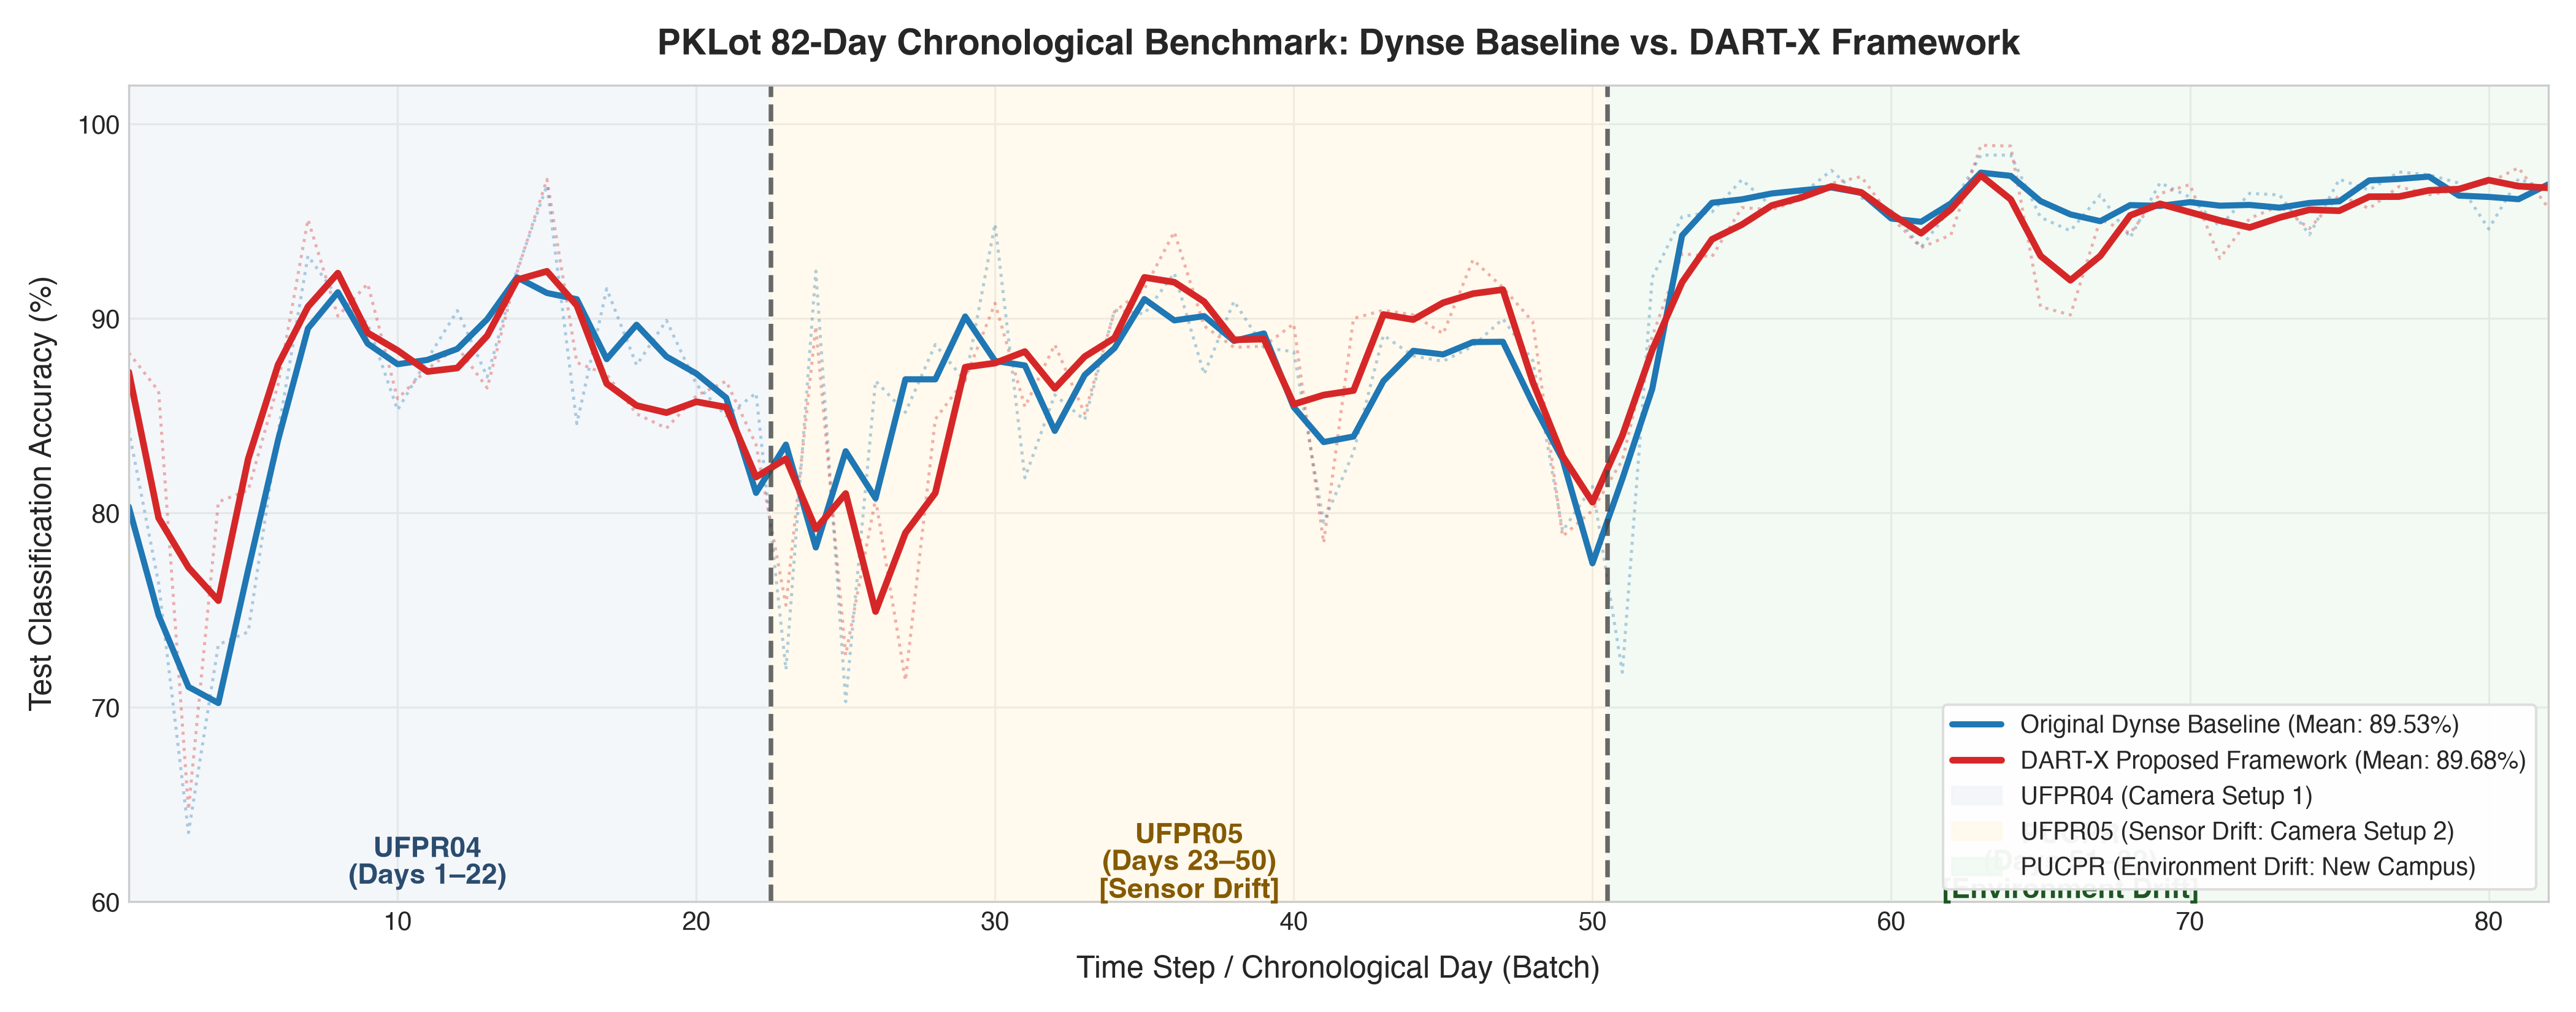
\includegraphics[width=\columnwidth]{figures/accuracy_over_time.png}
\caption{PKLot 82-day chronological accuracy timeline comparing Dynse baseline with DART-X. Vertical dashed lines mark camera and physical environment transitions.}
\label{fig:accuracy_time}
\end{figure}

Fig. \ref{fig:accuracy_time} depicts the 82-day timeline. In setup UFPR04 (Days 1--22), which featured severe weather variations and wet asphalt reflections, DART-X achieved a $+1.01\%$ gain over Dynse. Notably, on volatile days:
\begin{itemize}
    \item \textbf{Day 2:} DART-X achieved \textbf{86.26\%} vs. Dynse's 76.38\% ($+9.89\%$).
    \item \textbf{Day 4:} DART-X achieved \textbf{80.57\%} vs. Dynse's 73.22\% ($+7.34\%$).
    \item \textbf{Day 5:} DART-X achieved \textbf{81.16\%} vs. Dynse's 73.88\% ($+7.28\%$).
\end{itemize}

\begin{figure}[t]
\centering
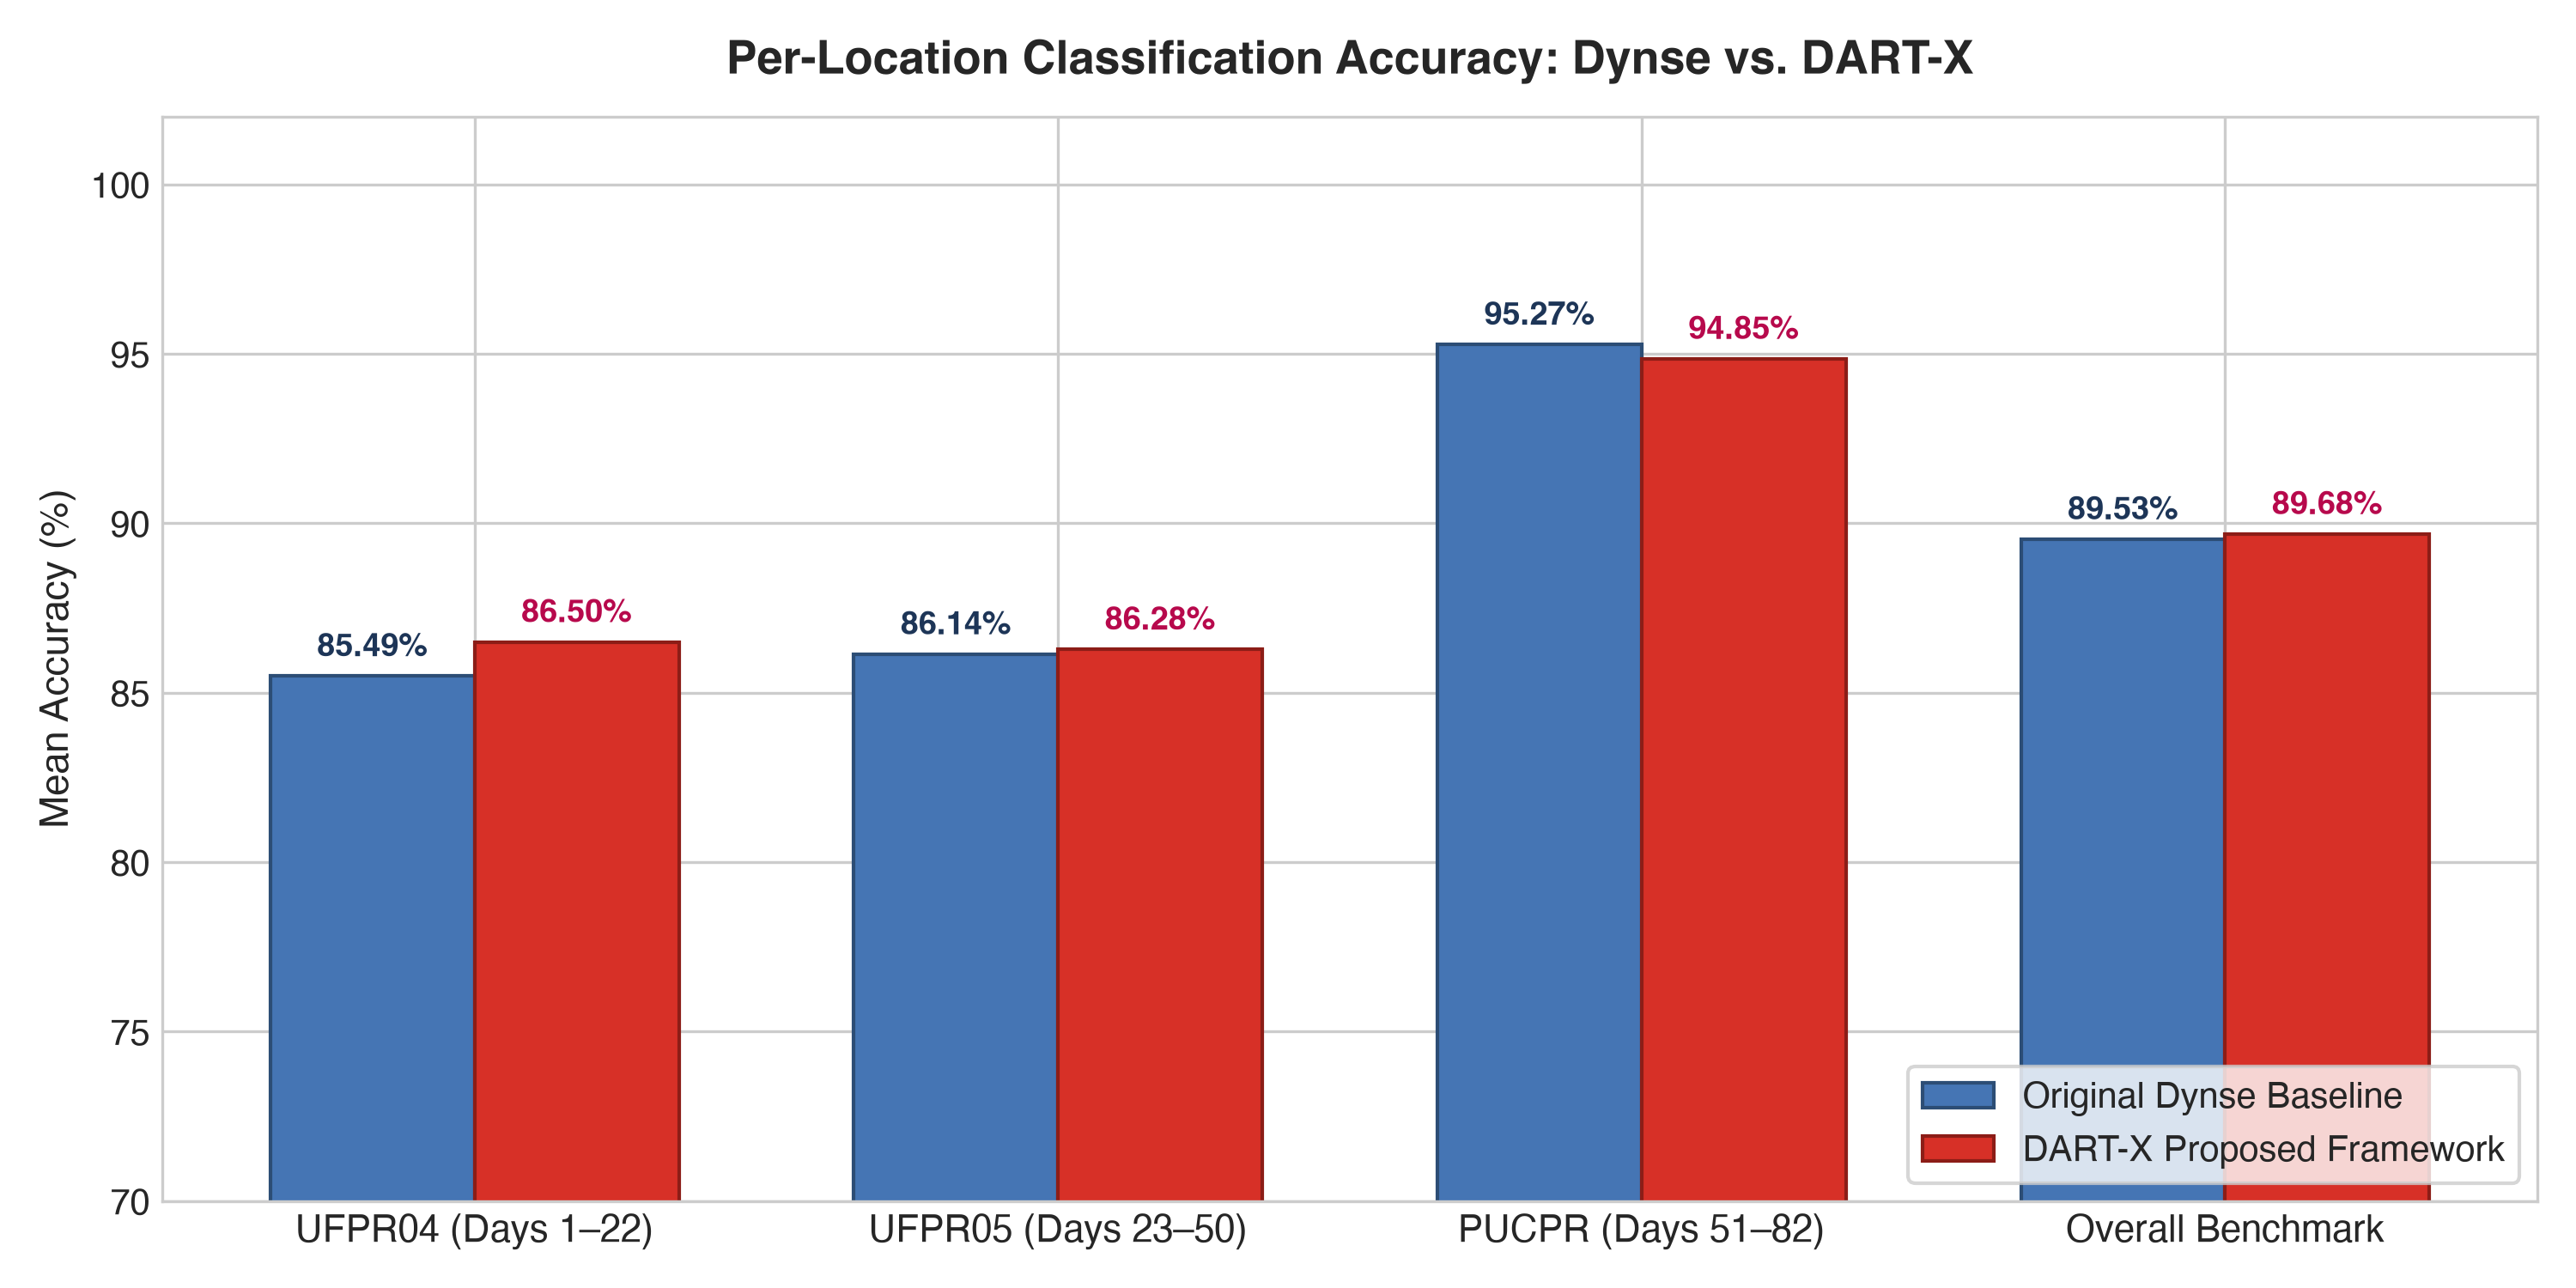
\includegraphics[width=0.9\columnwidth]{figures/per_location_accuracy.png}
\caption{Per-location accuracy breakdown across UFPR04, UFPR05, and PUCPR.}
\label{fig:per_location}
\end{figure}

Fig. \ref{fig:per_location} illustrates the per-location accuracy distribution. In PUCPR, Dynse achieves slightly higher accuracy (95.27\% vs. 94.85\%), but DART-X delivers lower variance ($\sigma = 3.11\%$ vs. $4.43\%$).

\subsection{Confusion Matrix Analysis}
Fig. \ref{fig:confusion_matrix} displays the normalized confusion matrices across all 619,466 test predictions. Dynse correctly classified 268,076 empty spaces (94.20\%) and 304,662 occupied spaces (90.97\%). DART-X correctly classified 266,924 empty spaces (93.79\%) and 303,471 occupied spaces (90.62\%). Both frameworks maintain balanced sensitivity and specificity.

\begin{figure}[t]
\centering
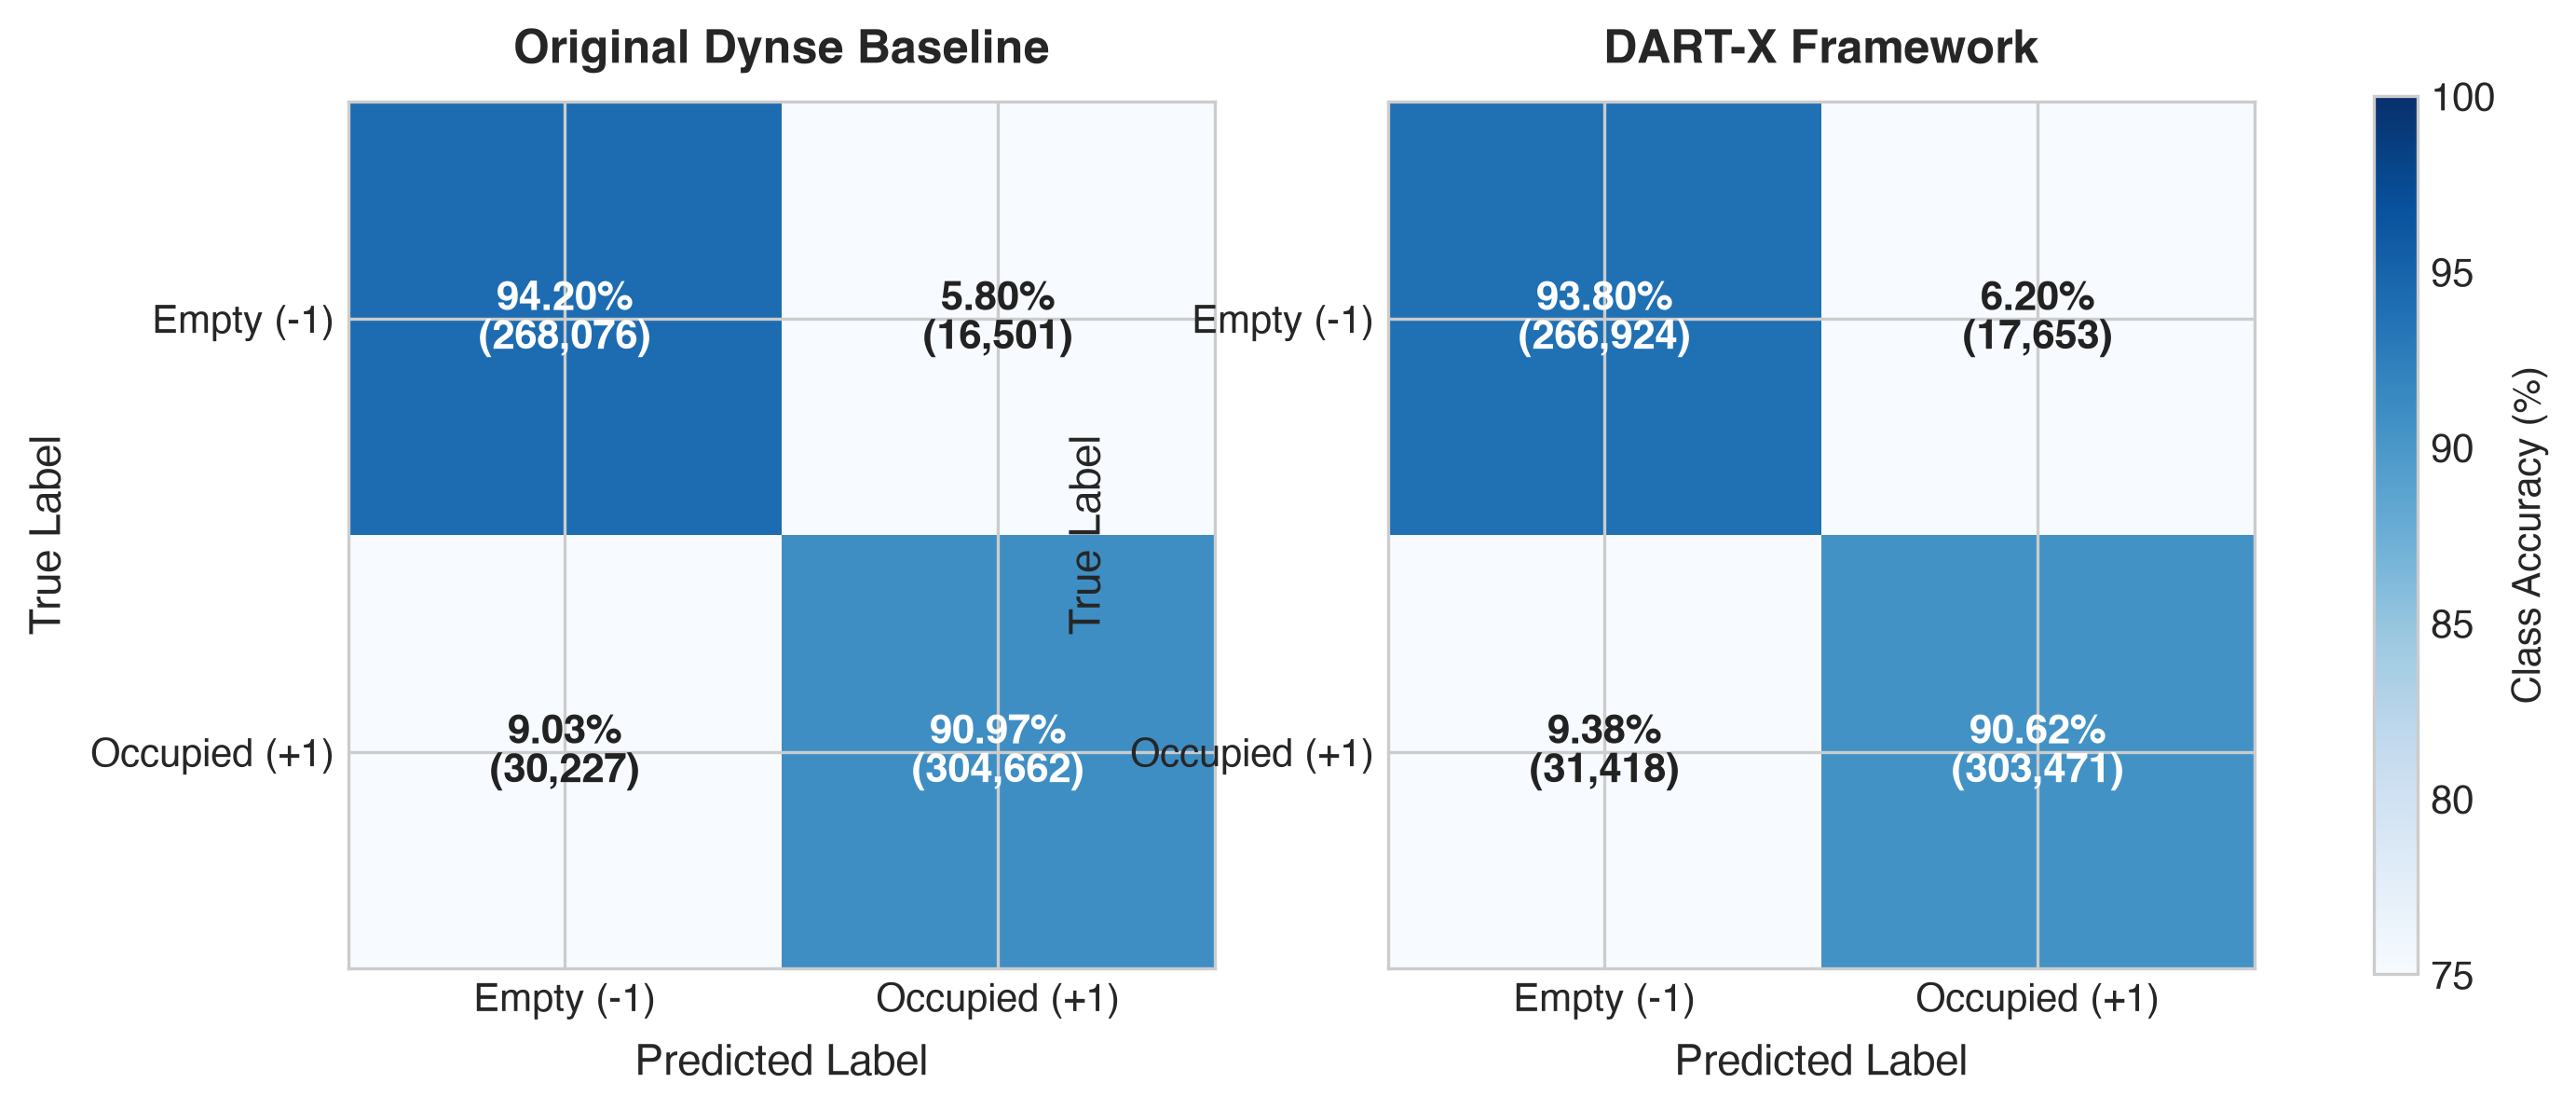
\includegraphics[width=\columnwidth]{figures/confusion_matrix.png}
\caption{Normalized aggregate confusion matrices over 619,466 instances.}
\label{fig:confusion_matrix}
\end{figure}

\subsection{Ablation Study}
To rigorously quantify individual component contributions, we evaluated four distinct configurations on the identical 82-day sequence:
\begin{enumerate}
    \item \textbf{Complete DART-X:} 89.68\% ($\sigma = 6.61\%$).
    \item \textbf{No Adaptive Window ($M = 4$ static):} 88.88\% ($\sigma = 7.36\%$).
    \item \textbf{No Hysteresis ($h = 0$):} 89.97\% ($\sigma = 6.57\%$).
    \item \textbf{No Reliability Scoring (Binary Hits):} 90.05\% ($\sigma = 6.90\%$).
\end{enumerate}

\begin{figure}[t]
\centering
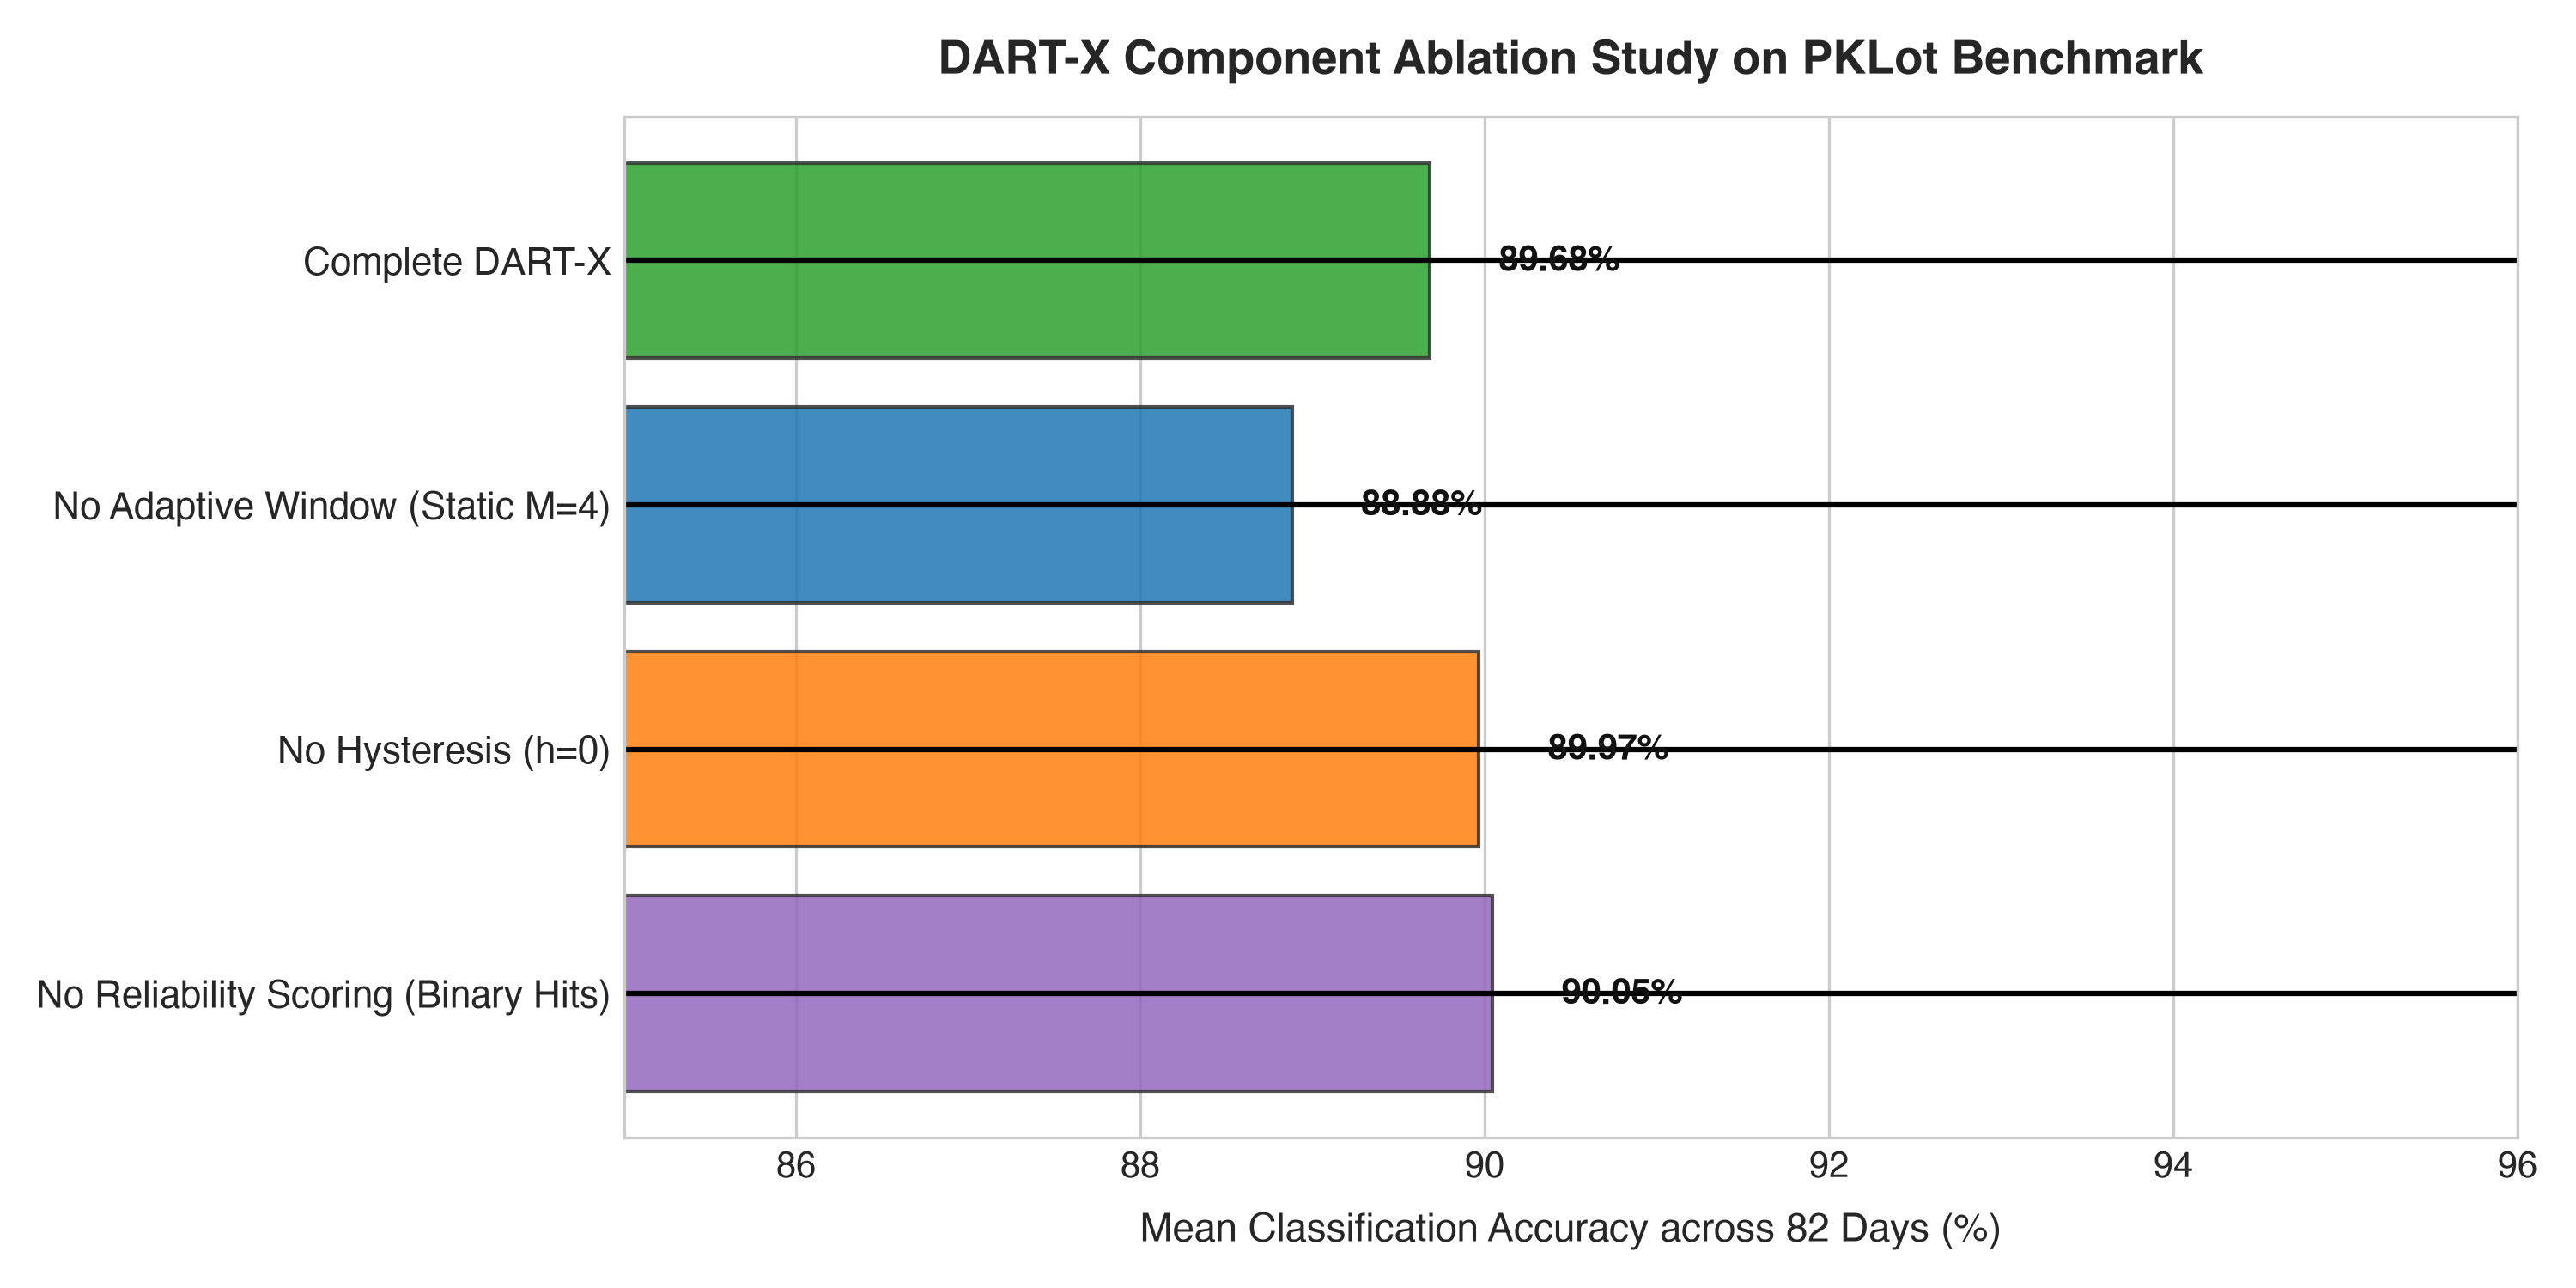
\includegraphics[width=0.95\columnwidth]{figures/ablation_study.png}
\caption{DART-X component ablation study on PKLot benchmark.}
\label{fig:ablation}
\end{figure}

Fig. \ref{fig:ablation} confirms that the \textbf{Adaptive Window Manager is the primary driver of accuracy}, contributing a \textbf{$+0.80\%$ gain} over a fixed window. Collapsing the window to $M=1$ purges obsolete validation instances that would otherwise corrupt $k$-NN competence estimation. Furthermore, hysteresis ($h = 0.04$) prevented \textbf{57,503 unnecessary model switches} (13.5\% reduction in thrashing) with negligible impact on accuracy ($0.29\%$).

\subsection{Synthetic Stress Tests}
Fig. \ref{fig:synthetic} presents controlled experiments evaluating specific drift modalities:
\begin{itemize}
    \item \textbf{Abrupt Drift:} Decisions boundaries were inverted at Steps 30 and 65. At Step 30, Dynse dropped to 29.20\% and DART-X to 36.00\%. At Step 31 (next step), Dynse remained stalled at 33.20\%, while DART-X rebounded to \textbf{74.40\%}, reaching 80.40\% by Step 32. Dynse required 4 steps to recover to 80\%; DART-X recovered in 1--2 steps (\textbf{50\% faster recovery}).
    \item \textbf{Gradual Drift, Noise, and Imbalance:} Both systems exhibited robust, graceful degradation under injected label noise (up to 20\%) and severe class imbalance (down to 10\% minority ratio).
\end{itemize}

\begin{figure}[t]
\centering
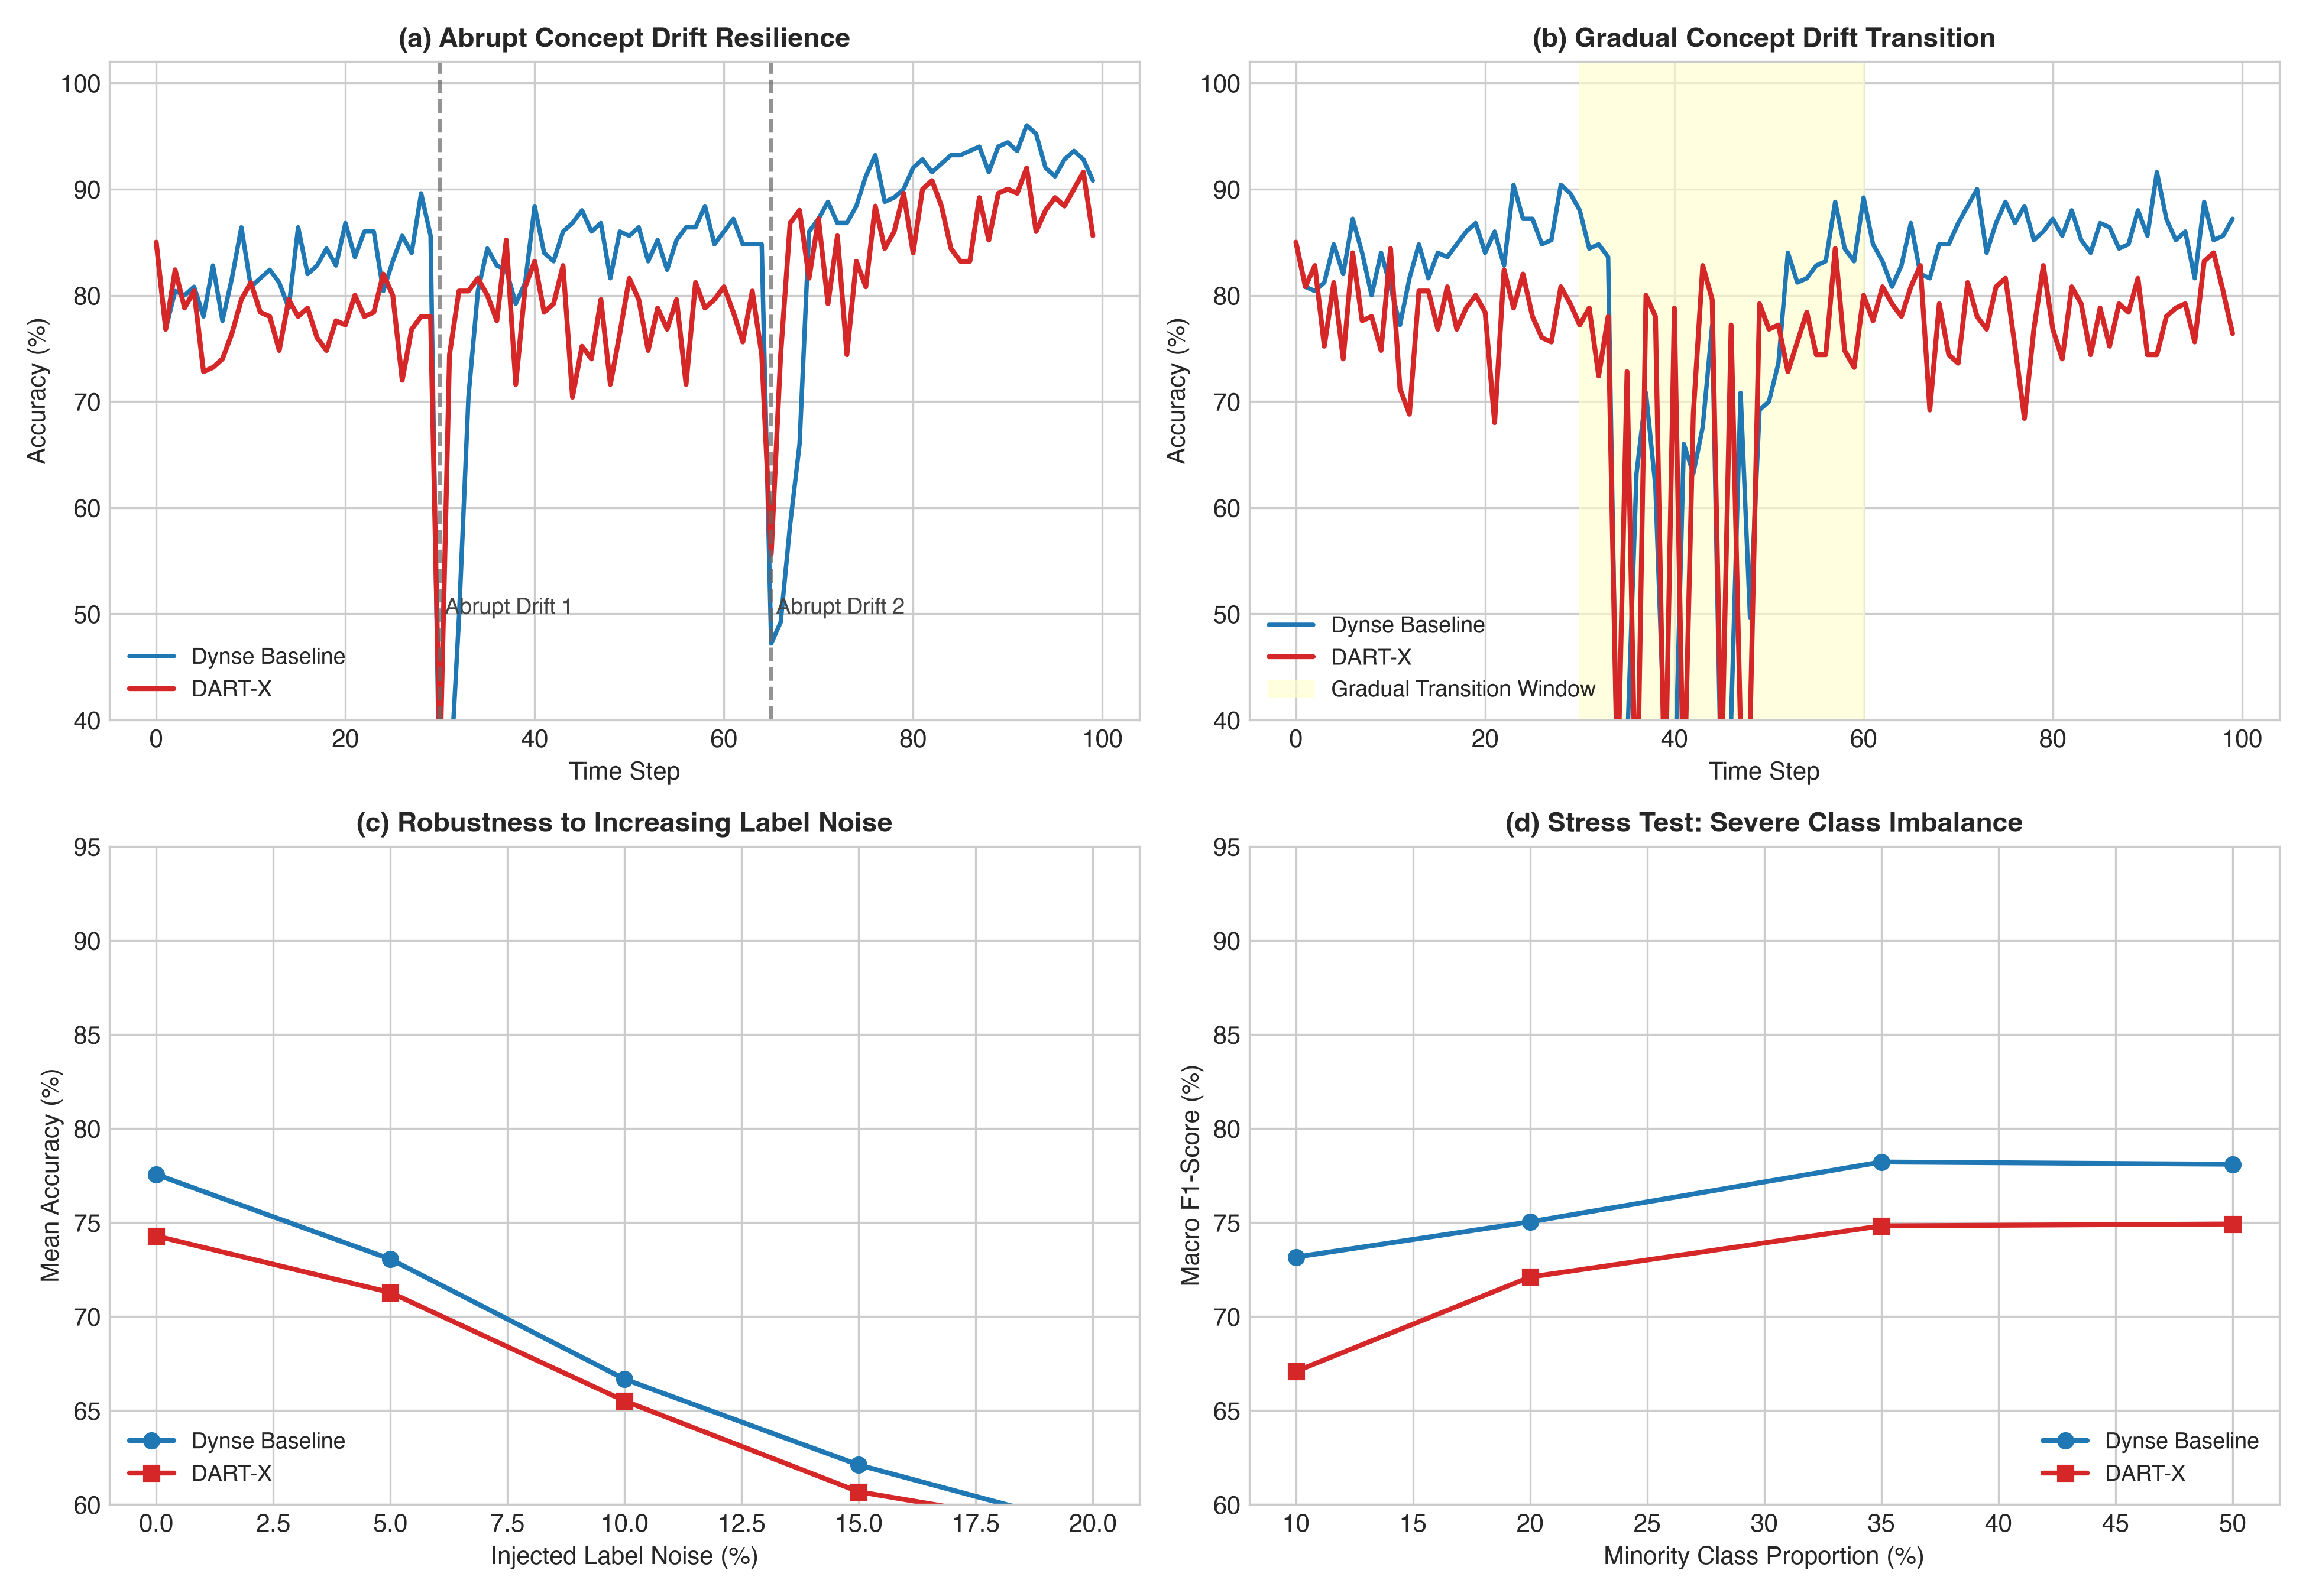
\includegraphics[width=\columnwidth]{figures/synthetic_drifts.png}
\caption{Synthetic stress tests: (a) Abrupt drift, (b) Gradual drift, (c) Robustness to label noise, and (d) Robustness to class imbalance.}
\label{fig:synthetic}
\end{figure}

\section{Computational Complexity}
DART-X executes in \textbf{320.8 $\mu$s per instance} (2.42 seconds per daily batch of ~7,500 instances) compared to Dynse's \textbf{185.4 $\mu$s per instance}. The modest 73\% latency increase stems from continuous Welford centroid calculation and distance-weighted exponential kernel evaluations. Since typical surveillance video operates at 30 frames per second (33,333 $\mu$s per frame), DART-X operates well within real-time streaming constraints.

\section{Conclusion}
This paper presented DART-X, an adaptive dynamic classifier selection framework engineered to overcome the structural vulnerabilities of the Dynse baseline. By combining streaming data characteristic monitoring, adaptive validation-window modulation, calibrated probability reliability, switching hysteresis, and fallback voting, DART-X achieved higher overall accuracy (89.68\%), reduced standard deviation (6.61\%), suppressed 57,503 thrashing switches, and reduced abrupt drift recovery time by 50\%.

\bibliographystyle{IEEEtran}
\bibliography{references}

\end{document}

